\documentclass{esannV2}
\usepackage{graphicx}
\usepackage[utf8]{inputenc}
\usepackage{amssymb,amsmath,array}

\usepackage{hyperref}
\usepackage{listings}
\lstset{
  language=bash,
  basicstyle=\ttfamily
}
%***********************************************************************
% !!!! IMPORTANT NOTICE ON TEXT MARGINS !!!!!
%***********************************************************************
%
% Please avoid using DVI2PDF or PS2PDF converters: some undesired
% shifting/scaling may occur when using these programs
% It is strongly recommended to use the DVIPS converters, and to submit
% PS file. You may submit a PDF file if and only if you use ADOBE ACROBAT
% to convert your PS file to PDF.
%
% Check that you have set the paper size to A4 (and NOT to letter) in your
% dvi2ps converter, in Adobe Acrobat if you use it, and in any printer driver
% that you could use.  You also have to disable the 'scale to fit paper' option
% of your printer driver.
%
% In any case, please check carefully that the final size of the top and
% bottom margins is 5.2 cm and of the left and right margins is 4.4 cm.
% It is your responsibility to verify this important requirement.  If these margin requirements and not fulfilled at the end of your file generation process, please use the following commands to correct them.  Otherwise, please do not modify these commands.
%
\voffset 0 cm \hoffset 0 cm \addtolength{\textwidth}{0cm}
\addtolength{\textheight}{0cm}\addtolength{\leftmargin}{0cm}

%***********************************************************************
% !!!! USE OF THE esannV2 LaTeX STYLE FILE !!!!!
%***********************************************************************
%
% Some commands are inserted in the following .tex example file.  Therefore to
% set up your ESANN submission, please use this file and modify it to insert
% your text, rather than staring from a blank .tex file.  In this way, you will
% have the commands inserted in the right place.

\begin{document}
%style file for ESANN manuscripts
\title{El título que queráis}

%***********************************************************************
% AUTHORS INFORMATION AREA
%***********************************************************************
\author{Jorge Durán León, Jaime Enríquez Ballesteros, Marcos de las Heras Roncero
%
% Optional short acknowledgment: remove next line if non-needed
%\thanks{This is an optional funding source acknowledgement.}
%
% DO NOT MODIFY THE FOLLOWING '\vspace' ARGUMENT
\vspace{.3cm}\\
%
% Addresses and institutions (remove "1- " in case of a single institution)
  Escuela Politécnica Superior, Fundamentos de Aprendizaje Automático \\
%Address of First Author's school - Country of First Author's
%school
%
% Remove the next three lines in case of a single institution
%\vspace{.1cm}\\
%2- School of Second Author - Dept of Second Author \\
%Address of Second Author's school - Country of Second Author's school\\
}
%***********************************************************************
% END OF AUTHORS INFORMATION AREA
%***********************************************************************

\maketitle

\begin{abstract}
Resumen del trabajo realizado en 100 palabras.
\end{abstract}

\section{Introducción}

El proyecto que se ha realizado trata sobre el análisis de un conjunto de datos recogidos por 8 sensores de gas, un sensor de temperatura y un sensor de humedad. Estos sensores fueron expuestos a estímulos por la presencia de vino y plátanos. Además, se recogen datos de la respuesta a la no presencia de ninguno de ellos. El objetivo del proyecto es la clasificación de las respuestas de los sensores a los estímulos previamente dichos. Para ello primero se analizarán los datos del dataset mediante técnicas de preprocesamiento para ver que pueden ofrecer esos datos a la hora de clasificar las respuestas. Después, se elegirán los modelos de aprendizaje automático supervisado que mejor nos convengan para dicho dataset. Por último, se compararán los resultados de los distintos modelos y razonaremos si son resultados aceptables y qué modelos han dado mejores resultados.

\section{Descripción del dataset}
El dataset proporcionado de los datos de los sensores está compuesto por dos archivos: el archivo HT\_Sensor\_dataset.dat; que contiene el identificador de la inducción, instantes de tiempo para cada inducción y los datos de los sensores para cada inducción en esos instantes de tiempo, y el archivo HT\_Sensor\_metadata.dat; que contiene para cada inducción su identificador, el día en que fue realizada, el estímulo usado para la inducción, y el intervalo de tiempo de la inducción, que está dividido en tiempo inicial y duración de la misma. \\
En este último dataset hay 3 clases distintas para clasificar, que se corresponden con los estímulos que reciben los sensores:  vino (wine), plátano (banana) y ningún estímulo (background). En total se realizan 100 inducciones, donde  36 se realizan con vino, 33 con plátano y 31 son background. De esas 100 inducciones se recogen 928991 datos en distintos instantes de tiempo. Al analizar los datos se puede comprobar que no hay datos para la inducción con el identificador 95, por lo que esta instancia es descartada del análisis. Además de los datos recogidos durante la inducción, se nos ofrecen los datos de los instantes previos y posteriores de la inducción. Esta división del tiempo se puede calcular fácilmente para cada inducción con la ayuda de los datos del tiempo del archivo de los metadatos (HT\_Sensor\_metadata.dat), por lo que podemos distinguir para cada experimento estos tres periodos diferenciados. Comprobamos que para los experimentos con identificadores 14 y 76 no tenemos datos posteriores a la inducción, por lo que también los descartamos, quedando 97 instancias válidas. \\
Los atributos del dataset son numéricos y reales, por lo que se pueden utilizar las medidas características de la distribución de cada atributo para analizarlo. Estas medidas pueden ser de centralización, como la media, o de dispersión, como la varianza. Con estas medidas se puede ver como se comporta cada sensor frente a los estímulos. En el siguiente apartado se verá un pequeño resumen sobre el  análisis llevado a cabo sobre los datos y el proceso a seguir para obtener los atributos que serán utilizados para entrenar a los modelos en el apartado 4.

\section{Análisis  de los datos}
La mayoría de funciones utilizadas para el análisis de los datos y el preprocesamiento previo al entrenamiento de modelos se pueden encontrar en el fichero \textit{Preprocess.py}. La única excepción es la función utilizada para la representación de instancias a lo largo del tiempo que encontramos en el fichero \\ \textit{Plot\_Induction\_Figure.py} que se facilita en [1]. Se utilizan los módulos de Pandas, NumPy, Sci-kit Learn y Matplotlib. \\
El primer paso para el análisis será representar los experimentos para cada clase y fijarse en qué atributos pueden marcar la diferencia a la hora de clasificar. La Figura~\ref{fig:banvswinvsbck} muestra al progresión de los sensores para 3 experimentos (id=0, id=1, id=69), uno por clase.

\begin{figure}[b!]
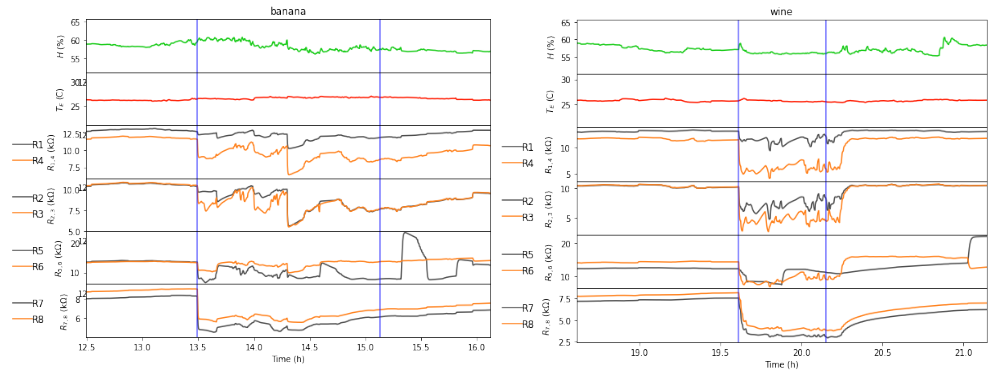
\includegraphics[scale=0.35]{img/banvswin.png}
\centering
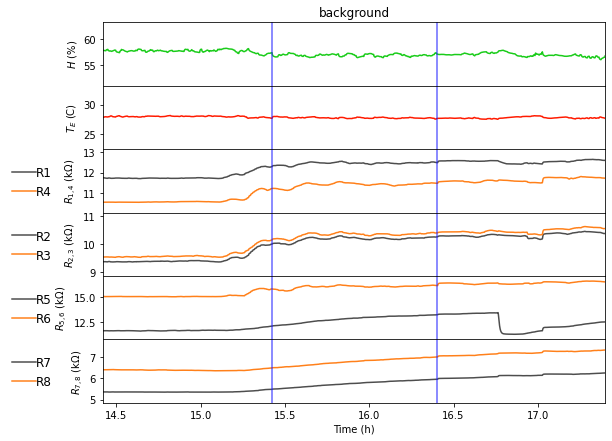
\includegraphics[scale=0.3]{img/background_69.png}
\caption{Comparación entre clases}\label{fig:banvswinvsbck}
\end{figure}


Se puede observar como los atributos de temperatura y humedad obtienen valores  y varianzas muy similares independientemente de la clase. En la Figura ~\ref{fig:tempvshum} comprobamos como estos atributos no nos van a ayudar a predecir la clase de cada experimento, al no estar correlacionados. Por otro lado, observamos como cuando la humedad es más alta, los sensores obtienen unos resultados más fluctuantes que con humedad baja. Se puede ver claramente cuando se representan los experimentos con id=0 e id=10 (en Notebook).

\begin{figure}[b!]
\centering
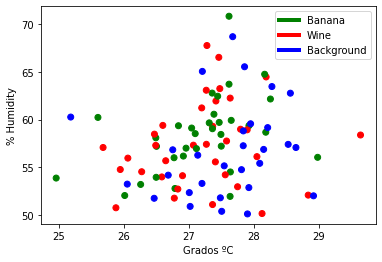
\includegraphics[scale=0.5]{img/temp_hum.png}
\caption{Temperatura y. Humedad respecto a clases}\label{fig:tempvshum}
\end{figure}

Por otro lado, los sensores obtienen estimulaciones muy diferentes entre ellos según la clase. La fluctuación de los sensores durante la estimulación del experimento (entre las dos líneas azules)  es muy pronunciada para el vino, seguido del plátano y muy poco notable cuando no se introduce ningún elemento en el sensor. En la Figura~\ref{fig:banvswinvsbck} se muestra muy claramente. Por lo tanto, la varianza de cada sensor puede ser un posible atributo para nuestro modelo. \\
Además, como se muestra en el notebook, la media y mediana de los sensores son muy similares independientemente de la clase que utilicemos. Esto significa que no serán atributos útiles para el modelo final.


\section{Modelos y Atributos propuestos}

- Atributo x atributo posible. Por qué y por qué no

- Lazy predict

- Modelos elegidos

\section{Discusión de resultados}



\section{Memoria}
La longitud máxima serán \emph{8 caras} sin incluir referencias. Se valorará la
capacidad de síntesis por lo que superar las 8 páginas tendrá penalización. La
memoria se deben tratar, de forma orientativa, los siguientes aspectos:

\begin{itemize}
\item Introducción [1pt]: breve introducción al problema a analizar, descripción del dataset y objetivos.
\item Análisis exploratorio de los datos [1pt]: Descripción estadística de los datos: Número de clases, distribución de las clases, otras estadísticas y análisis.
\item Descripción de los distintos atributos  propuestos y cómo se obtienen [2pt]
Modelos utilizados, descripción del protocolo experimental, estimación de parámetros, etc [2pt]: En esta sección se debe especificar toda la información necesaria para que otra persona, sin acceso a vuestro código, pueda reproducir los experimentos que habéis hecho. Debe quedar claro en la descripción que no se usan los datos de test para entrenar los modelos.
\item Resultados obtenidos en forma tabular y/o usando gráficas [1pt]. Se debe describir que muestra cada tabla o gráfica.
\item Discusión de los resultados obtenidos y conclusiones [2pt] Esta sección es la más importante del documento ya que es dónde se pone en valor el trabajo realizado. Debéis responder a preguntas  tipo ¿Qué atributos y métodos han dado mejores resultados? ¿Por qué creéis que es así? ¿Son resultados aceptables? ¿Qué modelos recomendaríais bajo qué condiciones? Tal vez un modelo funcione mejor cuando se entrena con pocos datos o funcione mejor para clasificar una de las clases y peor para otras, etc.
\item Además se deben utilizar al menos dos de las técnicas descritas a los largo del curso por vuestros compañeros [1pt]
\end{itemize}

Se valorará la correcta redacción del documento.

\section{Presentación}
Debéis entregar un ppt o pdf con el resumen del trabajo. Debe ser una
presentación para presentar en 12 minutos. El tiempo de presentación será
estricto y se parará a los que se pasen de tiempo.

\section{Tablas y figuras}
Las tablas y figuras hay que referenciarlas desde el texto y describir qué
muestran. Por ejemplo, en la Figura~\ref{fig:logo} se muestra el logo de
scikit-learn. En la Tabla~\ref{tab:ageweight} se muestra un ejemplo de tabla.


\begin{figure}[b!]
\centering
%\includegraphics{logo.png}
\caption{Logo de scikit-learn}\label{fig:logo}
\end{figure}

\begin{table}[t!]
  \centering
  \begin{tabular}{|c|c|c|}
    \hline
    ID & age & weight \\
    \hline
    1& 15 & 65 \\
    2& 24 & 74\\
    3& 18 & 69 \\
    4& 32 & 78 \\
    \hline
  \end{tabular}
  \caption{Age and weight of people.}\label{tab:ageweight}
\end{table}

\section{Citas}
Es una buena práctica referenciar los trabajos en los que se ha basado vuestro
análisis. Por ejemplo, si los experimentos se han realizado utilizado
scikit-learn habría que citarlo~\cite{scikit-learn}.

\section{Cómo obtener este pdf usando \LaTeX}
Podéis seguir los siguientes pasos para obtener el pdf junto con sus
referencias desde una consola linux:

\begin{lstlisting}
 pdflatex fuente.tex
 bibtex fuente
 pdflatex fuente.tex
 pdflatex fuente.tex
\end{lstlisting}

Estos comandos generan el fichero pdf que incluye las referencias. Las
referencias se guardan en un fichero aparte (en esta caso mi\_bibliografia.bib).
% ****************************************************************************
% BIBLIOGRAPHY AREA
% ****************************************************************************

\begin{footnotesize}

% IF YOU DO NOT USE BIBTEX, USE THE FOLLOWING SAMPLE SCHEME FOR THE REFERENCES
% ----------------------------------------------------------------------------
%\begin{thebibliography}{99}
%
% For books
%\bibitem{Haykin_book} S. Haykin, editor. \emph{Unsupervised Adaptive Filtering vol.1 : Blind Source Separation}, John Willey ans Sons, New York, 2000.
%
% For articles
%\bibitem{DelfosseLoubaton_article}N. Delfosse and P. Loubaton, Adaptibe blind separation of sources: A deflation
%approach, \emph{Signal Processing}, 45:59-83, Elsevier, 1995.
%
%% For paper in proceedings published as serie books (LNCS,...)
%\bibitem{CrucCichAmari_bookproceedings} S. Cruces, A. Cichocki and S. Amari, The minimum entropy and cumulants based contrast functions for blind source extraction. In J. Mira and A. Prieto, editors, proceedings of the 6$^{th}$ \emph{international workshop on artificial neural networks} ({IWANN} 2001), Lecture Notes in Computer Science 2085, pages 786-793,
%Springer-Verlag, 2001.
%
%% For paper in conference proceedings
%\bibitem{VrinsArchambeau_proceedings} F. Vrins, C. Archambeau and M. Verleysen, Towards a local separation performances estimator using common ICA contrast functions? In M. Verleysen, editor, \emph{proceedings of the $12^{th}$
%European Symposium on Artificial Neural Networks} ({ESANN} 2004),
%d-side pub., pages 211-216, April 28-30, Bruges (Belgium), 2004.
%
%% For Technical Report
%\bibitem{Stone_TechRep} J. V. Stone and J. Porrill, Undercomplete independent component analysis for signal separation and dimension
%reduction. Technical Report, Psychology Department, Sheffield
%University, Sheffield, S10 2UR, England, October 1997.
%\end{thebibliography}
% ----------------------------------------------------------------------------

% IF YOU USE BIBTEX,
% - DELETE THE TEXT BETWEEN THE TWO ABOVE DASHED LINES
% - UNCOMMENT THE NEXT TWO LINES AND REPLACE 'Name_Of_Your_BibFile'

\bibliographystyle{unsrt}
\bibliography{mi_bibliografia}

\end{footnotesize}

% ****************************************************************************
% END OF BIBLIOGRAPHY AREA
% ****************************************************************************

\end{document}
